\title{INVOLUTIONS AND SINGULARITIES}
\markright{Involutions and Singularities}

\author{By~~ F. Hirzebruch and K. J\"anich\footnote{Presented by F. Hirzebruch}}

\date{}

\maketitle

\setcounter{pageoriginal}{218}
\section{Introduction}\label{art10-sec1}\pageoriginale

Let $X$ be a compact oriented differentiable manifold without boundary of dimension $4k-1$ with $k\geq 1$. Let $T:X\to X$ be an orientation preserving fixed point free differentiable involution. In \cite{art11-key7} an invariant $\alpha(X,T)$ was defined using a special case of the Atiyah-Bott-Singer fixed point theorem. If the disjoint union $mX$ of $m$ copies of $X$ bounds a $4k$-dimensional compact oriented differentiable manifold $N$ in such a way that $T$ can be extended to an orientation preserving involution $T_{1}$ on $N$ which may have fixed points, then
\begin{equation}
\alpha(X,T)=\dfrac{1}{m}(\tau(N,T_{1})- \tau(\Fix T_{1}\circ \Fix T_{1})).\label{art11-sec1-eq1}
\end{equation}
Here $\tau(N,T_{1})$ is the signature of the quadratic form $f_{T_{1}}$ defined over $H_{2k}(N,\bfQ)$ by
$$
f_{T_{1}}(x,y)=x\circ T_{1}y
$$
where ``$\circ$'' denotes the intersection number. $\tau(\Fix T_{1}\circ \Fix T_{1})$ is the signature of the ``oriented self-intersection cobordism class'' $\Fix T_{1}\circ \Fix T_{1}$. According to Burdick \cite{art11-key4} there exist $N$ and $T_{1}$ with $m=2$.

In \S\ref{art11-sec2} we shall study a compact oriented manifold $\mathscr{D}$ whose boundary is $X-2(X/T)$. This manifold $\mathscr{D}$ was first constructed by Dold \cite{art11-key5}; we give a different description of it. Namely, $\mathscr{D}$ is a branched covering of degree $2$ of $(X/T)\times I$, where $I$ is the unit interval. The covering transformation is an orientation preserving involution $T_{1}$ of $\mathscr{D}$ which restricted to the boundary is $T$ on $X$ and the trivial involution on $2(X/T)$, and $\Fix T_{1}$ is the branching locus.

We show that
$$
\alpha(X,T)=\tau(\mathscr{D},T_{1})=-\tau(\mathscr{D}),
$$\pageoriginale
where $\tau(\mathscr{D})$ is the signature of the $4k$-dimensional manifold $\mathscr{D}$. Thus $\alpha(X,T)$ is always an integer. The construction of $\mathscr{D}$ is closely related to Burdick's result on the oriented bordism group of $B_{Z_{2}}$ and can in fact be used to prove it.

In \cite{art11-key7} it was claimed that if $X^{4k-1}$ is an integral homology sphere then $\tau(\mathscr{D})=\pm \beta(X,T)$, where $\beta(X,T)$ is the Browder-Livesay invariant \cite{art11-key3}. The proof was not carried through. It turns out that the definition of Browder-Livesay is also meaningful without assumptions on the homology of $X$. In \S\ref{art11-sec3} we shall prove
\setcounter{equation}{2}
\begin{equation}
\beta(X,T)=-\tau(\mathscr{D}).\label{art11-sec1-eq3}
\end{equation}
By \eqref{art11-sec1-eq2}, we obtain
\begin{equation}
\alpha(X,T)=\beta(X,T).\label{art11-sec1-eq4}
\end{equation}
Looking at $\mathscr{D}$ as a branched covering of $(X/T)\times I$ has thus simplified considerably the proof of \eqref{art11-sec1-eq4} envisaged in \cite{art11-key7}.

If $a=(a_{0},a_{1},\ldots,a_{2k})\in \bfZ^{2k+1}$ with $a_{j}\geq 2$, then the affine algebraic variety
\begin{equation}
z^{a_{0}}_{0}+z^{a_{1}}_{1}+\cdots+z^{a_{2k}}_{2k}=0\label{art11-sec1-eq5}
\end{equation}
has an isolated singularity at the origin whose ``neighborhood boundary'' is the Brieskorn manifold \cite{art11-key1}
$$
\Sigma^{4k-1}_{a}\subset C^{2k+1}
$$
given by the equation \eqref{art11-sec1-eq5} and 
\begin{equation}
\sum\limits^{2k}_{i=0}z_{i}\overline{z}_{i}=1.\label{art11-sec1-eq6}
\end{equation}
If all the $a_{j}$ are odd, then $Tz=-z$ induces an orientation preserving fixed point free involution $T_{a}$ on $\sigma_{a}$. The calculation of $\alpha(\Sigma_{a},T_{a})$ is an open problem (compare \cite{art11-key7}). This problem on isolated singularities is the justification for presenting out paper to a colloquium on algebraic geometry. In \S\ref{art11-sec4} we give the recipe for calculating $\alpha(\Sigma_{a},T_{a})$ for $k=1$ in the case where the exponents $a_{0}$, $a_{1}$, $a_{2}$ are pairwise prime and odd.

\section{The Dold construction}\label{art11-sec2}\pageoriginale

Let $Y$ be a compact differentiable manifold without boundary and $W$ a 1-codimensional compact submanifold with boundary $\partial W$. Then, as it is well known, one can construct a double covering of $Y$, branched at $\partial W$, by taking two copies of $Y$, ``cutting'' them along $W$ and then identifying each boundary point of the cut in copy one with its opposite point in copy two. The same can be done if $Y$ is a manifold with boundary and $W$ intersects $\partial Y$ transversally in a union of connected components of $\partial W$. The covering will then be branched at $\partial W-\partial W\cap \partial Y$.

We are interested in a very special case of this general situation. Let $M$ be a compact differentiable manifold without boundary and $V$ a closed submanifold without boundary of codimension 1 in $M$. Then we define $Y=M\times [0,1]$ and $W=V\times [0,\frac{1}{2}]$.
\begin{figure}[H]
\centering
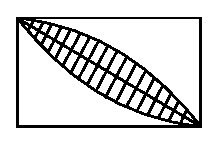
\includegraphics{figures/fig1.eps}
\end{figure}

For the following we will need a detailed description of the double covering corresponding to $(M\times [0,1],V\times [0,\frac{1}{2}])$. The normal bundle of $V$ in $M$ defines a $\bfZ_{2}$-principal bundle $\widetilde{V}$ over $V$. If we ``cut'' $M$ along $V$, we obtain a compact differentiable manifold $C$ with boundary $\partial C=\widetilde{V}$. As a set, $C$ is the disjoint union of $M-V$ and $\widetilde{V}$, and there is an obvious canonical way to introduce topology and differentiable structure in $(M-V)\cup \widetilde{V}$. Similarly, let $C'$ be the disjoint union of $M\times [0,1]-V\times [0,\frac{1}{2})$ and $\widetilde{V}\times [0,\frac{1}{2})$, topologized in the canonical way. Then we consider two copies $C'_{1}$ and $C'_{2}$ of $C'$ and identify in their disjoint union each $x\in V\times \{\frac{1}{2}\}\subset C'_{1}$ with the corresponding point $x\in V\times \{\frac{1}{2}\}\subset C'_{2}$ and for $0\leq t<\frac{1}{2}$ each point $v\in \widetilde{V}\times \{t\}\subset C'_{1}$ with the opposite point $-v\in \widetilde{V}\times \{t\}\subset C'_{2}$. Let $\mathscr{D}$ denote\pageoriginale the resulting topological space and $\pi:\mathscr{D}\to M\times [0,1]$ the projection. Then $C'_{1}$, $C'_{2}$ and $V\times \{\frac{1}{2}\}$ are subspaces, and $\mathscr{D}-V\times \{\frac{1}{2}\}$ has a canonical structure as a differentiable manifold with boundary.

To introduce a differentiable structure on all of $\mathscr{D}$, we use a tubular neighbourhood of $V$ in $M$. This may be given as a diffeomorphism
$$
\kappa : \fprod{\widetilde{V}}{D^{1}}{Z_{2}}\to M
$$
onto a closed neighbourhood of $V$ in $M$, such that the restriction of $\kappa$ to $\fprod{\widetilde{V}}{\{0\}}{Z_{2}}=V$ is the inclusion $V\subset M$. Let $Z_{2}$ act on $D^{2}\subset \bfC$ by complex conjugation. Then we get a tubular neighbourhood of $V\times \{\frac{1}{2}\}$ in $M\times [0,1]$
\setcounter{equation}{0}
\begin{equation}
\begin{split}
&\lambda : \fprod{\widetilde{V}}{D^{2}}{Z_{2}}\to M\times [0,1]\quad\text{by}\\
&[v,x+iy]\mapsto (\kappa(v,y),\frac{1}{2}+\frac{1}{4}x).
\end{split}
\label{art11-sec2-eq1}
\end{equation}
Let the ``projectin'' $p:\fprod{\widetilde{V}}{D^{2}}{Z_{2}}\to \fprod{\widetilde{V}}{D^{2}}{Z_{2}}$ be given on each fibre by $z\to z^{2}/|z|$. Then $\lambda p$ can be lifted to $\mathscr{D}$, which means that we can choose a map $\lambda_{1}:\fprod{\widetilde{V}}{D^{2}}{Z_{2}}\to \mathscr{D}$ such that
\begin{equation}
\vcenter{\xymatrix{
\fprod{\widetilde{V}}{D^{2}}{Z_{2}}\ar[d]^-{p}\ar[r]^-{\lambda_{1}} & \mathscr{D}\ar[d]^-{\pi}\\
\fprod{\widetilde{V}}{D^{2}}{Z_{2}}\ar[r]^-{\lambda} & M\times [0,1]
}}\label{art11-sec2-eq2}
\end{equation}
is commutative. Then there is exactly one differentiable structure on $\mathscr{D}$ for which $\lambda_{1}$ is a diffeomorphism onto a neighborhood of $V\times \{\frac{1}{2}\}$ in $\mathscr{D}$ and which coincides on $\mathscr{D}-V\times \{\frac{1}{2}\}$ with the canonical structure. Up to diffeomorphism, of course, this structure does not depend on $\kappa$.

$\mathscr{D}$, then, is a double covering of $M\times [0,1]$, branched at $V\times \{\frac{1}{2}\}$. The covering transformation on $\mathscr{D}$ shall be denoted by $T_{1}$. Note that on $\fprod{\widetilde{V}}{D^{2}}{Z_{2}}$ (identified by $\lambda_{1}$ with a subset of $\mathscr{D}$) the transformation $T_{1}$ is given by $[v,z]\to [v,-z]$.

As a differentiable manifold, $\mathscr{D}$ is the same as the manifold constructed by Dold in his note \cite{art11-key5}.

Now\pageoriginale 

